\documentclass[a4paper,12pt]{extarticle}
\usepackage{geometry}
\usepackage[T1]{fontenc}
\usepackage[utf8]{inputenc}
\usepackage[english,russian]{babel}
\usepackage{amsmath}
\usepackage{amsthm}
\usepackage{amssymb}
\usepackage{fancyhdr}
\usepackage{setspace}
\usepackage{graphicx}
\usepackage{colortbl}
\usepackage{tikz}
\usepackage{pgf}
\usepackage{subcaption}
\usepackage{listings}
\usepackage{indentfirst}
\usepackage[
backend=biber,
style=numeric,
maxbibnames=99
]{biblatex}
\addbibresource{refs.bib}
\usepackage[colorlinks,citecolor=blue,linkcolor=blue,bookmarks=false,hypertexnames=true, urlcolor=blue]{hyperref} 
\usepackage{indentfirst}
\usepackage{mathtools}
\usepackage{booktabs}
\usepackage[flushleft]{threeparttable}
\usepackage{tablefootnote}

\usepackage{chngcntr} % нумерация графиков и таблиц по секциям
\counterwithin{table}{section}
\counterwithin{figure}{section}

\graphicspath{{graphics/}}%путь к рисункам

\makeatletter
% \renewcommand{\@biblabel}[1]{#1.} % Заменяем библиографию с квадратных скобок на точку:
\makeatother

\geometry{left=2.5cm}% левое поле
\geometry{right=1.0cm}% правое поле
\geometry{top=2.0cm}% верхнее поле
\geometry{bottom=2.0cm}% нижнее поле
\setlength{\parindent}{1.25cm}
\renewcommand{\baselinestretch}{1.5} % междустрочный интервал


\newcommand{\bibref}[3]{\hyperlink{#1}{#2 (#3)}} % biblabel, authors, year
\addto\captionsrussian{\def\refname{Список литературы (или источников)}} 

\renewcommand{\theenumi}{\arabic{enumi}}% Меняем везде перечисления на цифра.цифра
\renewcommand{\labelenumi}{\arabic{enumi}}% Меняем везде перечисления на цифра.цифра
\renewcommand{\theenumii}{.\arabic{enumii}}% Меняем везде перечисления на цифра.цифра
\renewcommand{\labelenumii}{\arabic{enumi}.\arabic{enumii}.}% Меняем везде перечисления на цифра.цифра
\renewcommand{\theenumiii}{.\arabic{enumiii}}% Меняем везде перечисления на цифра.цифра
\renewcommand{\labelenumiii}{\arabic{enumi}.\arabic{enumii}.\arabic{enumiii}.}% Меняем везде перечисления на цифра.цифра

\begin{document}
\begin{titlepage}
    \newpage
    
    {\setstretch{1.0}
    \begin{center}
    ПРАВИТЕЛЬСТВО РОССИЙСКОЙ ФЕДЕРАЦИИ\\
    ФГАОУ ВО НАЦИОНАЛЬНЫЙ ИССЛЕДОВАТЕЛЬСКИЙ УНИВЕРСИТЕТ\\
    «ВЫСШАЯ ШКОЛА ЭКОНОМИКИ»
    \\
    \bigskip
    Факультет компьютерных наук\\
    Образовательная программа «Прикладная математика и информатика»
    \end{center}
    }
    
    \vspace{2em}
    УДК 004.421.2 % УДК нужно указывать только для исследовательсвого проекта - удалите эту строку для программного проекта
    \vspace{4em}
    
    \begin{center}
    %Выберите какой у вас проект
    {\bf Отчет об исследовательском проекте на тему:}\\
    %{\bf Отчет о командном исследовательском проекте на тему:}\\
    %{\bf Отчет о программном проекте на тему:}\\
    %{\bf Отчет о командном программном проекте на тему:}\\
    {\bf Гиперэвристика алгоритмов роевого интеллекта}\\
    % строчка ниже нужна только при сдача плана КР, при финальной сдаче закомментируйте ее
    (промежуточный, этап 1)
    \end{center}
    
    \vspace{2em}
    
    {\bf Выполнил студент: \vspace{2mm}}
    %{\bf Выполнили студенты: \vspace{2mm}}
    
    {\setstretch{1.1}
    \begin{tabular}{l@{\hskip 1.5cm}l}
    группы \#БПМИ236, 2 курса & Коростелев Данил Александрович \\
    %группы \#БПМИ172, 3 курса & Петров Андрей Алексеевич \\
    %группы \#БПМИ173, 3 курса & Иванов Андрей Алексеевич 
    \end{tabular}}
    
    % Обычно у вас есть один научный руководитель, и это человек, с которым вы работаете над проектом. Иногда по формальным причинам у вас будет руководитель (штатный сотрудник Вышки) и соруководитель (тот, с кем вы работаете), — об этом вам сообщит учебный офис (в случае с ВКР) или ЦППРиП (в случае с курсовым проектом). Также, если кто-то дополнительно вам помогал, то его можно указать как консультанта. 
    
    %ваш официальный научник (из ВШЭ)
    \vspace{1em}
    {\bf Принял руководитель проекта: \vspace{2mm}}
    
    {\setstretch{1.1}
    \begin{tabular}{l}
    Родригес Залепинос Рамон Антонио\\
    Научный сотрудник\\
    Факультет компьютерных наук НИУ ВШЭ 
    \end{tabular}}
    
    % со-руководитель (если есть)
    %\vspace{1em}
    %{\bf Соруководитель: \vspace{2mm}}%это ваш официальный научник
    
    %{\setstretch{1.1}
    %\begin{tabular}{l}
    %Петрова Надежда Александровна\\
    %Инженер-исследователь\\
    %ОАО Компания "Нейросети и деревья" 
    %\end{tabular}}
    
    % консультант (если есть)
    %\vspace{1em}
    %{\bf Консультант: \vspace{2mm}}%это ваш официальный научник
    
    %{\setstretch{1.1}
    %\begin{tabular}{l}
    %Иванова Надежда Александровна\\
    %Инженер-исследователь\\
    %ОАО Компания "Нейросети и деревья" 
    %\end{tabular}}
    
    \vspace{\fill}
    
    \begin{center}
    Москва 2024
    \end{center}
    
    \end{titlepage}% это титульный лист - выберите подходящий вам из имеющихся в проекте вариантов (kr - курсовая работа у 3 курса, vkr - выпускная квалификационная работа у 4 курса)
\newpage
\setcounter{page}{2}

{
	\hypersetup{linkcolor=black}
	\tableofcontents
}

\newpage

\newpage
\section*{Аннотация}   % this is how to use russian
Ваша аннотация на русском языке.

\addcontentsline{toc}{section}{Аннотация}

\section*{Ключевые слова}
Глубинное обучение, разреживание моделей, рекуррентные нейронные сети
\pagebreak

\section{Примеры} 
\subsection{Ссылки на статьи}

Ссылки на статьи оформляются с помощью пакета \texttt{biblatex}, например~\cite{chirkova18}. В описании статье в bib файле нужно обязательно указывать место публикации работы (журнал или конференцию) и год. Обратите внимание, что для описания статей из разных источников в списке литературы используются разные команды в bib файле: статья из журнала~\cite{ctan}, статья с конференции~\cite{chirkova18}, книга~\cite{knuth-acp}, глава книги~\cite{knuth-fa}. Если статься еще не опубликована нигде, а только выложена на arXiv, то на нее тоже можно сослаться~\cite{chirkova18_arxiv}, но предпочтительно ссылаться на опубликованную версию, если она уже существует. Если вы хотите сослаться на сайт, то можно либо так же внести его в список литературы~\cite{knuthwebsite} (рекомендуется, если таких ссылок у вас много из-за особенностей темы вашего проекта), либо использовать ссылку внизу страницы\footnote{Книги доступны по ссылке: \url{http://www-cs-faculty.stanford.edu/~uno/abcde.html}, дата обр. 16.05.2013}. При работе с онлайн ресурсами не забывайте указывать дату обращения к этому ресурсу, так как в отличие от опубликованных статей, эти ресурсы могут измениться в любой момент.

\subsection{Рисунки}

\begin{figure}[ht]
	\centering
	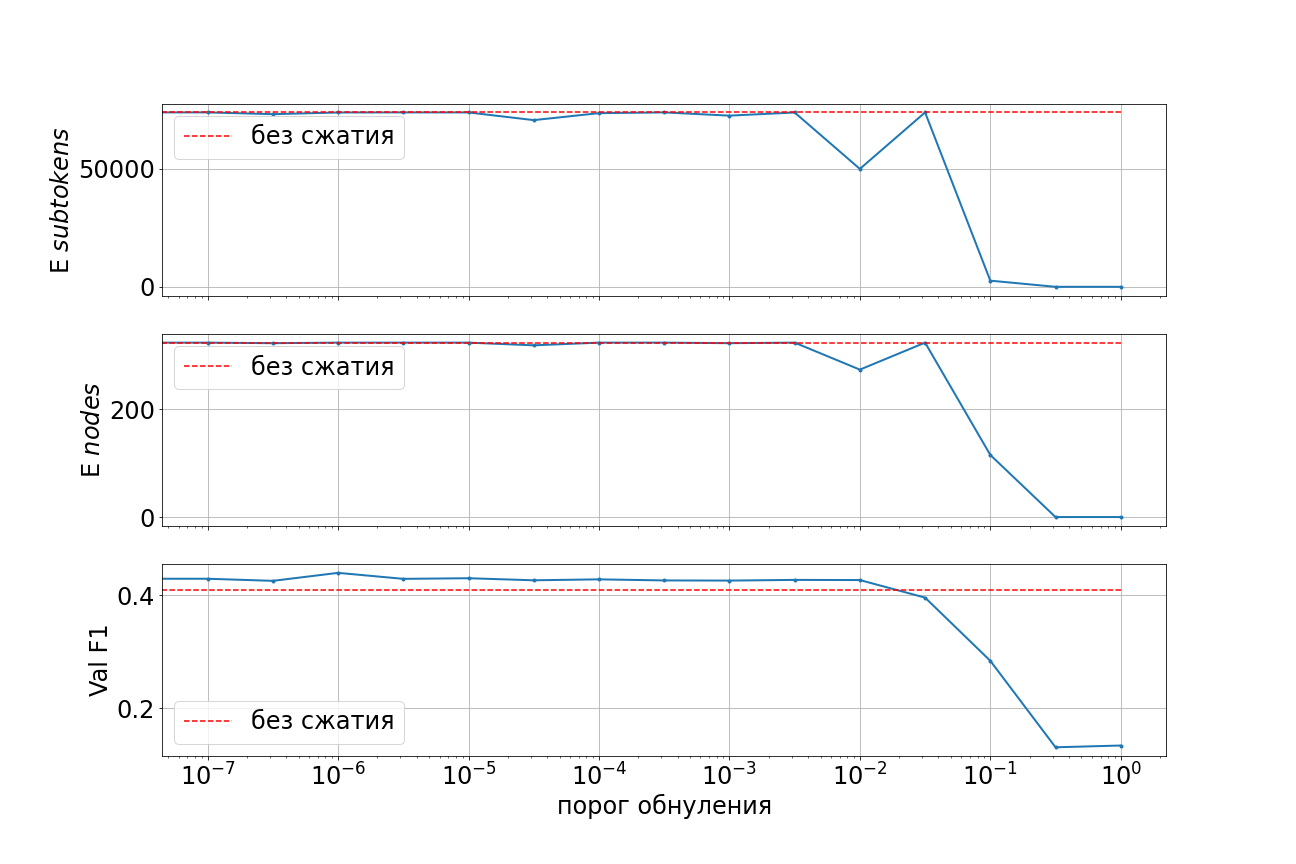
\includegraphics[width=0.8\textwidth]{example.png}
	\caption{Пример графика. Тут должна быть подпись, поясняющая что происходит на рисунке (краткая, но достаточная для понимания основной идеи графика).}
	\label{fig:by_epochs}
\end{figure}

Все рисунки в тексте должны иметь подписи и вы на них должны ссылаться в тексте. Например, на Рисунке~\ref{fig:by_epochs} изображен пример графика. Не забывайте подписывать все оси на графиках, добавлять легенду и пояснять все обозначения, а также используйте адекватного размера шрифты и толщину линий на графиках (все должно быть видно и понятно без многократного увеличения). На рисунке из примера явно не хватает обозначения синей линии в легенде.


\subsection{Таблицы}

Все таблицы в тексте тоже должны иметь подписи и вы на них должны ссылаться в тексте. Например, в Таблице~\ref{table:long_epochs} показаны результаты примерного эксперимента. 


\begin{table}[ht]
	\caption{Пример таблички. Тут должна быть подпись, поясняющая что происходит в таблице (краткая, но по делу).}
	\label{table:long_epochs}
	\footnotesize
	\centering
	\begin{tabular}{lrrrrrrrr}
		\toprule
		& \multicolumn{3}{c}{$\mathsf{Val}$} &
		\multicolumn{3}{c}{$\mathsf{Test}$} \\
		\cmidrule(lr){2-4} \cmidrule(l){5-7} 
		{} &  $\mathsf{Prec}$ &  $\mathsf{Rec}$ &  $\mathsf{F1}$ &  $\mathsf{Prec}$ &  $\mathsf{Rec}$ &  $\mathsf{F1}$  &  $\mathsf{nodes}$ & $\mathsf{subtokens}$\\
		\midrule
		запуск 1    &    0.4894 &   0.3775 &  0.4263 &     0.4824 &    0.3683 &   0.4177 & 10029 & 179\\
		запуск 2    &    0.4887 &   0.3739 &  0.4237 &     0.4891 &    0.3724 &   0.4228 & 10039 & 177\\
		запуск 3    &    0.4820 &   0.3751 &  0.4219 &     0.4838 &    0.3677 &   0.4178 & 10037&	180\\
		\midrule
		\bf{среднее} &    \bf{0.4867} &   \bf{0.3755} &  \bf{0.4239} &    \bf{ 0.4851} &    \bf{0.3695} &   \bf{0.4195} \\
		\bf{дисперсия}  &    0.0041 &   0.0019 &  0.0022 &     0.0036 &    0.0025 &   0.0029 \\
		\bottomrule
	\end{tabular}
\end{table}

\subsection{Формулы}

Формулы стоит центрировать, а также нумеровать, если вы ссылаете на них в тексте. Также не забывайте пояснять все обозначения в формулах. Например, запишем следующую задачу оптимизации:
\begin{equation}
    \label{eq:si_opt}
        \theta* = \min_{\theta} F(\theta),
\end{equation}
где $F$~-- квадратичная функция от параметра $\theta$. При необходимости, далее в тексте можно сослаться на формулу~(\ref{eq:si_opt}). При этом, в зависимости от конкретных формул, можно использовать разные слова: формула, уравнение, задача оптимизации и т.п.


	
\newpage 
\printbibliography[heading=bibintoc] 

% \begin{thebibliography}{0}
% 	\bibitem{chirkova18}\hypertarget{chirkova18}{}
% 	\href{https://arxiv.org/abs/1810.10927}
% 	{Nadezhda Chirkova, Ekaterina Lobacheva, Dmitry Vetrov. Bayesian Compression for Natural Language Processing. In EMNLP 2018.}
% \end{thebibliography}
	
\newpage
\appendix

\section{Пример секции аппендикса}

\end{document}
